\section{Performances de l'asservissement}
À chaque mouvement du sol, un capteur mesure la position angulaire du pendule (2) par rapport au bâti (1). Des bobines de contre-réaction situées sur le pendule (voir figure \ref{ccmp2023_fig_02} et l'Annexe 1) génèrent un moment de rappel sur son axe de rotation, qui le ramène à sa position d'équilibre.

\begin{itemize}
  \item La bobine HF (pour Haute Fréquence) pilote l'asservissement entre 0,05 Hz et 0,5 Hz. Son rôle principal est d'amortir les secousses trop brusques et d'éliminer la résonance du pendule.
  \item La bobine BF (pour Basse Fréquence) a été conçue pour intervenir sur les fréquences inférieures à $0,05 \si{Hz}$. Elle permet de filtrer la variation journalière de température et les dérives saisonnières plus lentes.
\end{itemize}

L'asservissement mis en place est donc une régulation devant permettre d'annuler en régime permanent les effets des secousses sismiques sur le pendule, tout en étant sensible aux signaux dans une large bande de fréquences d'ondes sismiques, entre $0,01 \si{Hz}$ et $0,5 \si{Hz}$.

Les exigences auxquelles doit répondre cet asservissement sont fournies dans la table \ref{ccmp2023_tab_03}.

\begin{table}[!h]
\centering
\begin{tabular}{cp{5cm}p{5cm}p{5cm}}
\hline
$\mathbf{3}$ & \multicolumn{3}{l}{Acquérir les vibrations du sol martien}  \\
\hline
$\mathbf{3.1}$ &\multirow{2}{4cm}{Éliminer la résonance du système tout en maintenant une rapidité maximale}&
Résonance du système avec l'action de la bobine HF seule &  aucune \\
\cline { 3 - 4 }
& & Rapidité du système avec l'action de la bobine HF seule & bande passante à $-3 \si{dB}$ maximale \\
\hline
$\mathbf{3 . 2}$ & 
Ramener le déplacement du pendule à zéro 
& Précision de l'asservissement en tension & écart statique nul en réponse à un échelon d'accélération du sol \\
\hline
$\mathbf{3 . 3}$ & Filtrer le signal & Amplification des mouvements du sol par l'asservissement en tension & 
$\geq 110 \si{dB}$ limitée à la bande $[0,06 ; 3]$ \si{rad} $\mathrm{s}^{-1}$ \\
\hline
$\mathbf{3 . 4}$ & Éviter des problèmes de saturation & Amplification des mouvements du sol par l'asservissement en tension 
&$<120 \si{dB}$ pour tous les signaux mesurés \\
\hline
\end{tabular}
\caption{\label{ccmp2023_tab_03}  Liste (non exhaustive) des exigences de l'asservissement}
%TABLE 3 - Liste (non exhaustive) des exigences de l'asservissement
\end{table}



\begin{obj}
Régler la correction des bobines $\mathrm{HF}$ et $\mathrm{BF}$.
\end{obj}

Le réglage de l'asservissement s'effectue par une étude numérique, dans les conditions de la gravité martienne. On considère donc le pendule (2) sans son contrepoids (3). On note $J$ le moment d'inertie du pendule (2) sur l'axe ( $\left.O_{1}, \overrightarrow{z_{1}}\right)$. Pour simplifier l'étude, on néglige les frottements dans l'articulation à lamelles, et on note $K=k-d M g_{M} \cos \alpha_{0}$ la raideur équivalente du pendule.

La grandeur utile aux scientifiques qui analysent les données mesurées par le sismomètre est la tension électrique en sortie du capteur, image de la position angulaire du pendule autour de sa position d'équilibre.

Le schéma-blocs de l'asservissement en tension d'un système est fourni en Annexe 5 , ainsi que la description des grandeurs physiques intervenant dans l'asservissement et les données numériques utiles à cette partie.

On s'intéresse dans un premier temps à l'asservissement avec l'action de la bobine HF seule. Le schéma-blocs correspondant est fourni à la figure \ref{ccmp2023_fig_11}.

\begin{figure}[!h]
\centering
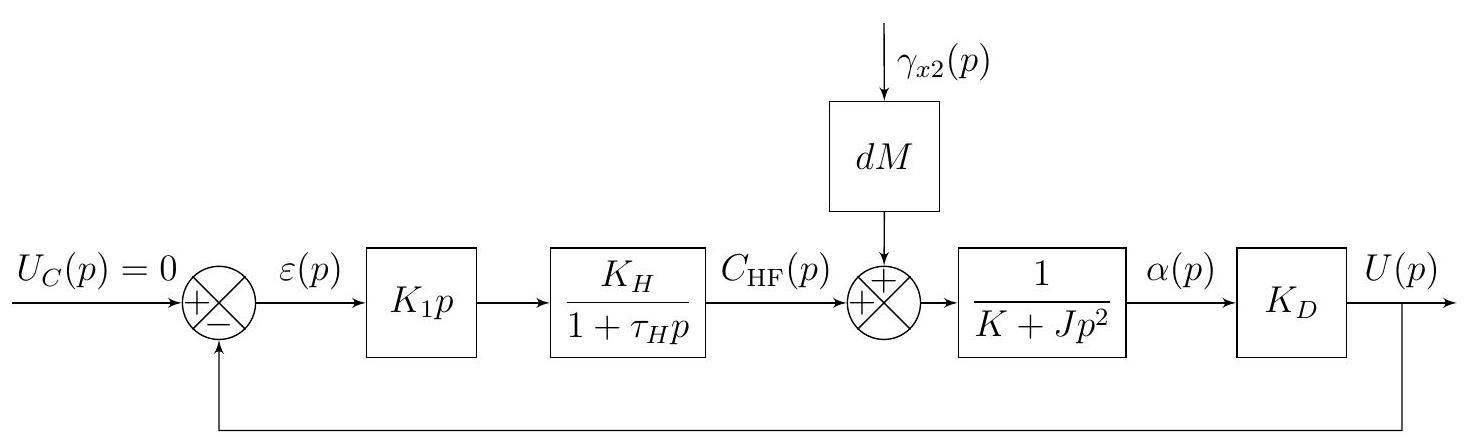
\includegraphics[width=\textwidth]{2024_04_26_3285cfc264024262add0g-13(1)}
\caption{\label{ccmp2023_fig_11} Schéma-blocs de l'asservissement avec l'action de la bobine HF seule}
\end{figure}

%FIGURE 11 - Schéma-blocs de l'asservissement avec l'action de la bobine HF seule

\question{\label{ccmp2023_q_23}. Déterminer la fonction de transfert $H_{\gamma}(p)=\frac{U(p)}{\gamma_{x 2}(p)}$, avec $U_{C}(p)=0$, en l'exprimant sous la forme:
$
H_{\gamma}(p)=K_{\mathrm{HF}} \cdot \frac{1+a_{1} p}{1+b_{1} p+b_{2} p^{2}+b_{3} p^{3}}
$
où l'on précisera les expressions de $K_{\mathrm{HF}}, a_{1}, b_{1}, b_{2}$ et $b_{3}$.}

On donne les pôles $p_{i}$ de $H_{\gamma}(p)$ en table \ref{ccmp2023_tab_04} et le diagramme de Bode en gain de $H_{\gamma}(p)$ en figure \ref{ccmp2023_fig_12} pour différentes valeurs de $K_{1}$.


\begin{table}[!h]
\centering
\begin{tabular}{|c|c|c|c|}
\hline
$K_{1}$ & $p_{1}$ & $p_{2}$ & $p_{3}$ \\
\hline\hline
0,05 & $-1000$ & $$-0,38-2,33$ \mathrm{j}$ & $-0,38+2,33 \mathrm{j}$ \\
\hline
0,5 & $-1000$ & $-0,64$ & $-9,32$ \\
\hline
5 & $-1000$ & $-0,069$ & $-95,7$ \\
\hline
\end{tabular}
\caption{\label{ccmp2023_tab_04} Pôles de la fonction de transfert $H_{\gamma}(p)$ }
\end{table}

%TABLE 4 - Pôles de la fonction de transfert $H_{\gamma}(p)$

\begin{figure}[!h]
\centering
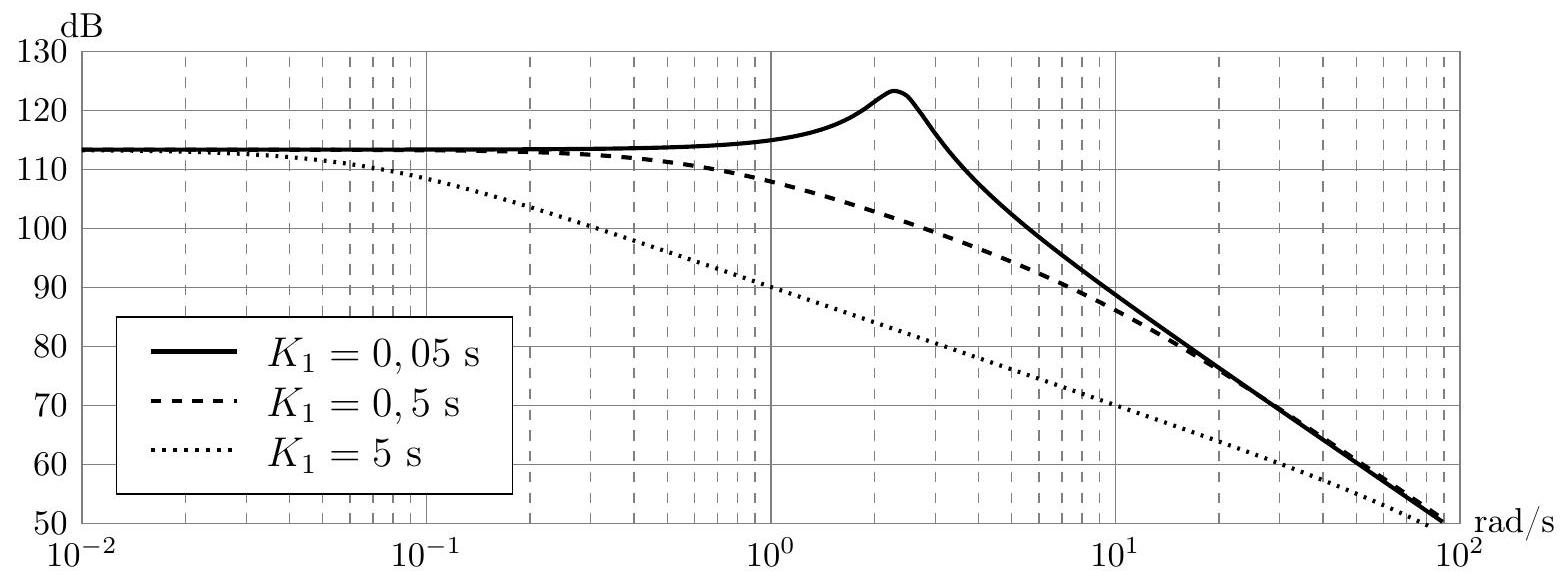
\includegraphics[width=\textwidth]{2024_04_26_3285cfc264024262add0g-13}
\caption{\label{ccmp2023_fig_12} Diagramme de Bode en gain de la fonction de transfert $H_{\gamma}(p)$}
%Figure 12 - Diagramme de Bode en gain de la fonction de transfert $H_{\gamma}(p)$
\end{figure}



Le réglage du correcteur HF doit permettre de répondre à l'exigence 3.1.

%Q24. 
\question{\label{ccmp2023_q_24}Justifier que $H_{\gamma}(p)$ correspond à un système stable quelle que soit la valeur retenue pour $K_{1}$ dans la gamme $[0,05 ; 5]$ s. Choisir, en justifiant, la valeur de $K_{1}$ parmi les valeurs proposées, la plus adaptée au réglage de l'asservissement avec l'action de la bobine HF seule.}

%Q25. 
\question{\label{ccmp2023_q_25}En s'appuyant sur les données numériques de la table \ref{ccmp2023_tab_04} et de l'Annexe 5, justifier que, pour la valeur retenue de $K_{1}$, la fonction de transfert peut s'écrire sous la forme :
$$
H_{\gamma}(p)=\frac{d M K_{D}}{K} \cdot \frac{1}{\left(1+\tau_{2} p\right)\left(1+\tau_{3} p\right)}, \text { avec } \tau_{2} \gg \tau_{3}
$$
Préciser les valeurs des constantes de temps $\tau_{2}$ et $\tau_{3}$.}

Pour la suite des questions, on conservera cette forme simplifiée de $H_{\gamma}(p)$.

%Q26. 
\question{\label{ccmp2023_q_26}Justifier que l'asservissement avec l'action de la bobine HF seule ne permet pas de satisfaire les exigences 3.2 et 3.3.}

En tenant compte des résultats précédents, le schéma-blocs de l'Annexe 5 peut se mettre sous la forme de celui de la Figure \ref{ccmp2023_fig_13}.

\begin{figure}[!h]
\centering
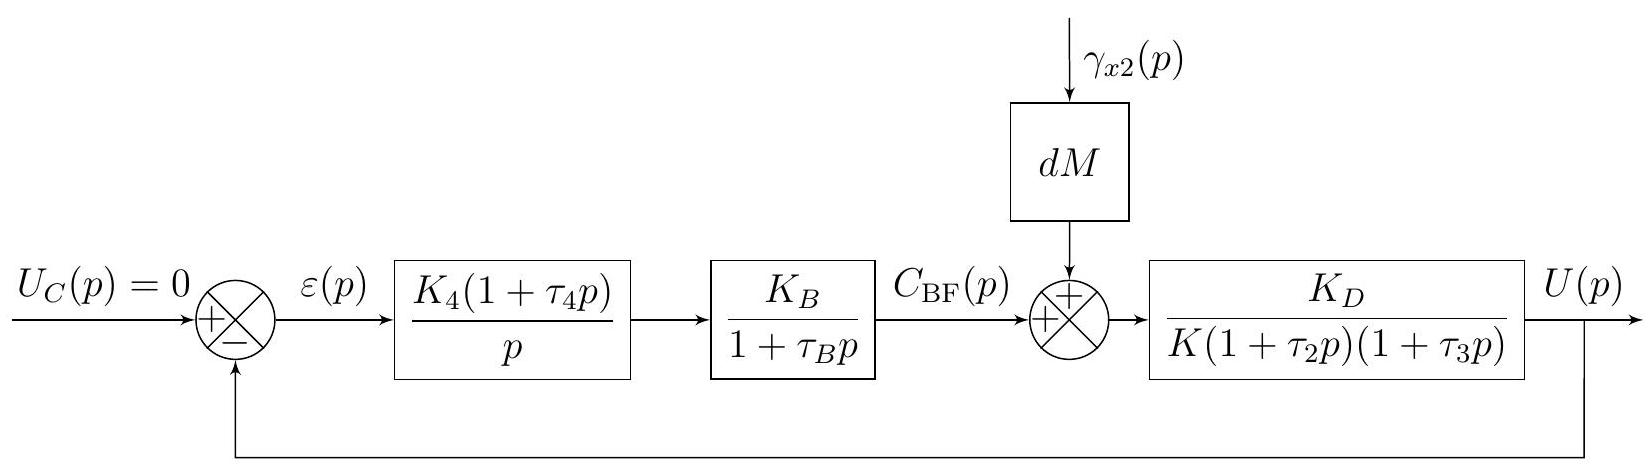
\includegraphics[width=\textwidth]{2024_04_26_3285cfc264024262add0g-14}
\caption{\label{ccmp2023_fig_13}  Schéma-blocs de l'asservissement d'un système}
%FigURe 13 - Schéma-blocs de l'asservissement d'un système
\end{figure}



Le correcteur BF est un correcteur proportionnel intégral. Pour optimiser la rapidité, $\tau_{4}$ doit permettre de compenser le pôle dominant de la boucle ouverte. $K_{4}$ est réglé de façon à répondre aux exigences 3.3 et 3.4.

%Q27. 
\question{\label{ccmp2023_q_27}Préciser l'intérêt de la chaîne d'action BF vis-à-vis de l'exigence 3.2.}

%Q28. 
\question{\label{ccmp2023_q_28}Donner l'expression de la fonction de transfert en boucle ouverte de l'asservissement, $H_{B O}(p)=\frac{U(p)}{\varepsilon(p)}$. Donner, en justifiant, la valeur retenue pour $\tau_{4}$.}

On donne, pour la valeur de $\tau_{4}$ retenue et différentes valeurs de $K_{4}$, le diagramme de Bode de l'asservissement en tension, $\frac{U(p)}{\gamma_{x 2}(p)}$, sur la Figure C du document réponse (question \ref{ccmp2023_q_29}).

%Q29. 
\question{\label{ccmp2023_q_29}Choisir, en justifiant, la valeur de $K_{4}$ qui permet de vérifier au mieux les exigences 3.3 et 3.4. Les tracés nécessaires apparaitront sur la document réponses.}

%Q30. 
\question{\label{ccmp2023_q_30}Donner le nom du type de filtre réalisé par le pendule asservi et préciser l'intérêt de cette solution pour la mesure des séismes par le sismomètre VBB.}
